\subsection{Modelo de Carga Potencial Máxima}
El objetivo de este modelo es seguir la evolución de la curva epidémica, y establecer predicciones a corto plazo $(t)$ de las cargas potenciales máximas de nuevos casos. El propósito de esto es estimar la saturación de un sistema de salud, lo que habilita una mejor toma de decisiones estratégicas de diverso tipo.

En este modelo, se establece que un nuevo caso tras un determinado tiempo $t$ es denominado como $C_t$, y existe un $I_t$ de personas infectadas, con $I_t = (C_t + C_{t-1})$. Estos casos, sin embargo, son puntos de transmisión de virus por hasta dos semanas, por lo que se puede establecer lo siguiente:

\begin{equation*}
    C_{t+1} \approx R_t (C_t + C_{t-1})
\end{equation*}

Esta expresión indica que todos los infectados en las dos semanas anteriores son contagiosos y van a contribuir a las infecciones del periodo $(t)$. Sin embargo, este no es el caso en la realidad, por lo que describir este proceso de transmisión en términos de probabilidad resulta más certero.

\begin{equation*}
    C_{t+1} =  \sum_{i=0}^{i=x} R_i p_i C_{tf - i} = R_t f(C_t + C_{t-1})
\end{equation*}

En esta expresión, $t$ es un periodo de tiempo, $i$ es una subdivisión de este periodo de tiempo, $tf$ es el último intervalo de este periodo, $p_i$ representa la probabilidad de que alguien infectado en el intervalo $tf-i$ infecte a alguien en el siguiente periodo de tiempo. Esto sugiere, entonces, una mejor expresión, tal que:

\begin{equation}
    C_{t+1} \approx fR_t (C_t + C_{t-1})
    \label{cpm_uno}
\end{equation}

En esta nueva expresión, $f$ corresponde a un factor de corrección como consecuencia de la distribución de probabilidad del intervalo serial. Para una carga máxima, este factor de corrección se estima como el máximo $p_i$.

\begin{figure}
    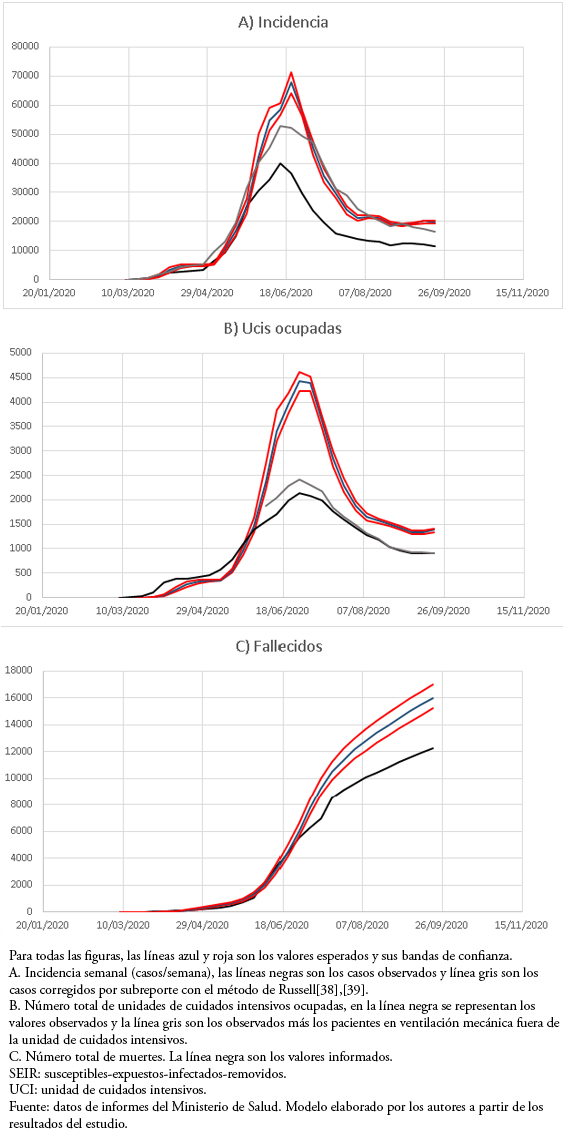
\includegraphics[width=\columnwidth]{cpm resultados.jpg}
    \caption{Resultados del uso del Modelo en el documento de Mauricio Canales y contribuidores. Fuente: \cite{canals_cuadrado_canals_2021}}
    \label{cpm resultados}
\end{figure}

Para el caso de Chile, los autores Mauricio Canales, Cristobal Cuadrado y Andrea Canales, desarrollaron este modelo con un periodo de tiempo $t$ equivalente a 1 semana. En este caso, el valor de $i$ corresponde a un día, y el valor de $x$ que se utiliza correspondería a 13, pues es la cantidad de tiempo que la persona enferma puede infectar, o sea, 2 semanas.

El desarrollo de este, se hizo con una distribución $\gamma$ con una media de 5 y una desviación estándar de $4,3$ días, por lo que su factor de corrección sería de $f \approx 0,8$. Bajo esto, generaron un modelo relativamente relacionado a la serie de Fibonacci, con dos valores iniciales. Para estos valores se utilizó $t_1 = 10$ y $t_2 = 65$, correspondientes a los casos nuevos en las primeras dos semanas de la epidemia.

Considerando que al rededor de un $3,5\%$ de los casos activos requiere tratamiento en una unidad de cuidados intensivos, y que estas suelen tener un estado de 'ocupadas' de dos semanas, y que la latencia entre el inicio de síntomas y el requerir una cama es de 1 semana, entregaron una expresión relacionada a la equación \eqref{cpm_uno} para predecir la cantidad de camas UCI ocupadas $U_t$:

\begin{equation}
    U_{t+1} = 0,035 (C_t + C_{t-1})
\end{equation}

En la figura \ref{cpm resultados} se observa los resultados de este modelo empleado por los autores, donde, pese a mantenerse certero en un inicio, termina sobre estimando los resultados de todos los parámetros que se intentaron predecir.